\documentclass[11pt,a4paper]{article}

\usepackage[T1]{fontenc}
\usepackage[utf8]{inputenc}
\usepackage{lmodern}
\usepackage[margin=0.9in]{geometry}
\usepackage{microtype}
\usepackage{graphicx}
\usepackage{booktabs}
\usepackage{tabularx}
\usepackage{array}
\usepackage{float}
\usepackage{caption}
\usepackage{subcaption}
\usepackage{xcolor}
\usepackage{xurl}
\usepackage{enumitem}
\usepackage{hyperref}
\usepackage{fancyhdr}
\usepackage{titlesec}
\usepackage{setspace}
\usepackage{needspace}
\usepackage{tikz}
\usetikzlibrary{arrows.meta,positioning,shapes.geometric}
\usepackage{longtable}
\usepackage{multirow}
\usepackage{amsmath}
\usepackage{amssymb}
\usepackage{listings}
\usepackage{colortbl}

\definecolor{patchblue}{HTML}{223A5E}
\definecolor{patchgreen}{HTML}{2F6F5E}
\definecolor{patchgray}{HTML}{555555}
\definecolor{lightblue}{HTML}{EAF1F8}
\definecolor{lightgreen}{HTML}{E8F3EE}
\definecolor{lightred}{HTML}{F8EAEA}

\hypersetup{
  colorlinks=true,
  linkcolor=patchblue,
  citecolor=patchgreen,
  urlcolor=patchblue,
  pdftitle={PatchPilot: A Safety-Constrained Tool-Using Agent for Python Debugging and Repair},
  pdfauthor={Tivdzua Lubem Noah and Gisele Wiykiynyuy},
  pdfkeywords={agentic AI, automated program repair, tool-using agents, hidden verification, mutation testing}
}

\setcounter{secnumdepth}{2}
\titleformat{\section}{\Large\bfseries\color{patchblue}}{\thesection}{0.7em}{}
\titleformat{\subsection}{\large\bfseries\color{patchgray}}{\thesubsection}{0.7em}{}
\titlespacing*{\section}{0pt}{0pt}{0.8em}
\titlespacing*{\subsection}{0pt}{1.2em}{0.45em}
\captionsetup{font=small,labelfont=bf}
\setlist[itemize]{leftmargin=1.35em,itemsep=0.2em,topsep=0.25em}
\setlist[enumerate]{leftmargin=1.6em,itemsep=0.2em,topsep=0.25em}
\renewcommand{\arraystretch}{1.16}
\setstretch{1.15}
\raggedbottom
\setlength{\headheight}{14pt}
\setlength{\emergencystretch}{2em}

\pagestyle{fancy}
\fancyhf{}
\lhead{PatchPilot}
\rhead{Research Project Report}
\cfoot{\thepage}

\newcommand{\code}[1]{\texttt{#1}}
\newcommand{\pp}{PatchPilot}

\begin{document}
\pagenumbering{gobble}

\begin{titlepage}
\centering
\vspace*{0.8cm}
{\Huge\bfseries PatchPilot\par}
\vspace{0.35cm}
{\LARGE A Safety-Constrained Tool-Using Agent for Python Debugging and Repair\par}
\vspace{0.8cm}
{\large Agentic AI Research Project Report\par}
\vspace{0.9cm}
\rule{0.82\textwidth}{0.5pt}\par
\vspace{0.55cm}
{\large\itshape
An evaluated repair prototype combining model-directed bounded tool use,
runtime-enforced safety constraints, transactional patching, hidden verification,
and trajectory-level analysis.\par}
\vspace{0.55cm}
\rule{0.82\textwidth}{0.5pt}\par
\vfill
\begin{tabular}{rl}
Team members: & Tivdzua Lubem Noah; Gisele Wiykiynyuy \\
Study type: & Experimental agentic software-repair prototype \\
Primary language: & Python \\
Model backend: & Ollama with \code{qwen2.5-coder:3b} \\
Evaluated commit: & \code{6524a37d802fc83faa9db0111facaf491da4e618} \\
Reporting/UI commit: & \code{c0ddba73d825d9e1262165328cec5b5786084266} \\
Evaluation matrix: & 53 tasks $\times$ 4 conditions = 212 runs \\
\end{tabular}
\vfill
{\large Final Report\par}
\vspace{0.2cm}
{\large July 15, 2026\par}
\vspace{0.8cm}
\parbox{0.86\textwidth}{\small
\textbf{Naming note.} This independently developed project predates the authors'
awareness of the unrelated 2025 research system also named PatchPilot by Li et al.
The distinction is stated explicitly in the related-work section.}
\end{titlepage}

\pagenumbering{arabic}
\section*{Abstract}
\addcontentsline{toc}{section}{Abstract}

PatchPilot is a bounded Agentic AI system for Python debugging and repair.
Given a task with failing tests, it prepares an isolated workspace, collects
execution evidence, permits a language model to select among dynamically
admissible repository tools, generates a source patch, checks syntax, and accepts
success only after executable verification of the current repository revision.
The runtime, rather than the model, owns safety-critical invariants: path
restrictions, exact tool-argument schemas, protected tests, execution budgets,
transactional rollback, stale-verification invalidation, and append-only traces.

The final evaluation contains 53 primary repair tasks: 45 mutation-generated
tasks and eight manually designed hard challenges. Four matched conditions were
run with the same local \code{qwen2.5-coder:3b} model: one-shot repair, a fixed
workflow, a tool-selecting agent without reflection, and a configured reflective
tool agent. All 212 runs completed. Hidden-verified repair rates were 69.8\% for
one-shot, 69.8\% for fixed workflow, 58.5\% for the non-reflective tool agent,
and 64.2\% for the reflective configuration. Cochran's $Q$ found global
heterogeneity ($Q(3)=11.0$, $p=0.0117$), but none of the six exact McNemar
comparisons remained significant after Holm correction. All conditions solved
0/8 hard manual challenges. Agentic variants were substantially slower, and the
final traces recorded no completed reflection or hypothesis-revision events.
Consequently, the experiment does not establish a causal benefit from
reflection. The primary engineering result is a safety-constrained, auditable, and
reproducible agent-computer interface. The evaluation indicates that additional
agency did not improve outcomes for this model and benchmark configuration.

\vspace{0.6em}
\noindent\textbf{Keywords:} agentic AI; automated program repair; tool-using agents; hidden verification; mutation testing; software safety.

\clearpage
\section{Introduction}

Modern code models can generate plausible source edits, but plausible text is
not equivalent to a verified repair. Software debugging is sequential and
environment-grounded: reproduce the failure, inspect evidence, form a
hypothesis, edit the correct source, and verify the current revision. If a patch
fails, the system must recover without weakening tests or accumulating unsafe
changes. This motivates an agent-environment design rather than a chatbot or
unrestricted code generator.

The original proposal specified a single-agent
Plan--Act--Observe--Reflect--Verify workflow with restricted tools, isolated
execution, rollback, budgets, and executable final verification. It also
proposed four conditions: one-shot, fixed workflow, tool use without reflection,
and the full reflective agent. The implemented project retains that experimental
structure while making the runtime boundary more explicit: the model has bounded
choice where choice is meaningful, while mandatory safety and verification
transitions remain deterministic.

The study addresses four research questions:

\begin{description}[leftmargin=0pt,labelindent=0pt]
  \item[RQ1.] How do the four repair-control strategies compare on
  hidden-verified repair success?
  \item[RQ2.] Does the configured reflective condition improve outcomes over
  tool use without reflection?
  \item[RQ3.] What latency, model-call, parsing, and trajectory costs accompany
  increasing agent autonomy?
  \item[RQ4.] Do runtime controls prevent invalid patches, unverified success,
  budget loops, and repeated no-progress behavior?
\end{description}

\clearpage
\section{Related Work and Conceptual Foundation}

\subsection{Reasoning, acting, and reflection}

ReAct interleaves reasoning with environment actions so that observations can
update subsequent decisions \cite{react}. Reflexion extends language agents
with verbal feedback from prior failures \cite{reflexion}. PatchPilot adopts
the same high-level interaction pattern, but it does not expose arbitrary shell
access and does not treat model prose as proof. Actions pass through a
schema-validated software interface, and completion is accepted only after tests
pass.

The evaluation framework used in the course distinguishes \emph{outcome} evaluation from
\emph{trajectory} evaluation: whether the final answer is correct versus
whether the agent used valid tools, efficient steps, safe actions, and reasonable
cost \cite{courseeval}. This distinction is central to the project because a
repair rate alone would hide argument-schema failures, unnecessary model calls,
latency, and the absence of actual reflection events.

\subsection{Software-engineering agents and benchmarks}

SWE-agent argues that agent-computer interface design can materially affect
software-engineering agent behavior \cite{sweagent}. PatchPilot follows this
principle with compact, task-specific actions, concise observations, exact
argument contracts, and runtime-owned transitions. SWE-bench provides an
execution-tested real-issue benchmark \cite{swebench}, while QuixBugs is a
small algorithmic repair benchmark with known overfitting risks
\cite{quixbugs}. The present study is intentionally smaller in repository
scale, but uses hidden execution tests and paired conditions to strengthen
internal validity.

A separate 2025 system is also named PatchPilot and reports a human-defined
reproduction--localization--generation--validation--refinement workflow
\cite{externalpatchpilot}. The project reported here is independent:
its repository, implementation, benchmark, and evaluation were developed for the
Agentic AI project. The shared name is acknowledged to avoid ambiguity.

\subsection{Model and mutation testing}

The experiment uses the 3B member of the Qwen2.5-Coder family, a code-specialized
open-weight model series \cite{qwen}. Mutation testing through \code{mutmut}
systematically generates executable defects; killed mutants are converted into
isolated repair tasks. Mutation tasks provide reproducible single-defect cases,
while the manual challenge set tests deeper stateful and multi-line logic beyond
simple operator mutations.

\clearpage
\section{System Design and Architecture}

\subsection{Bounded repair loop}

\begin{figure}[H]
\centering
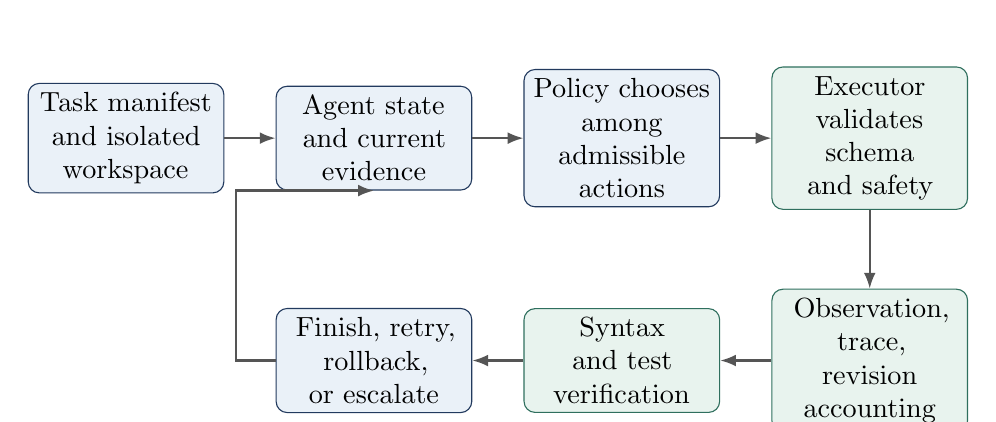
\begin{tikzpicture}[
  node distance=1.0cm and 0.65cm,
  box/.style={draw=patchblue,rounded corners,fill=lightblue,
    minimum height=1.0cm,text width=2.25cm,align=center},
  guard/.style={draw=patchgreen,rounded corners,fill=lightgreen,
    minimum height=1.0cm,text width=2.25cm,align=center},
  arrow/.style={-{Latex[length=2mm]},thick,draw=patchgray}
]
\node[box] (task) {Task manifest\\and isolated workspace};
\node[box, right=of task] (state) {Agent state\\and current evidence};
\node[box, right=of state] (policy) {Policy chooses among\\admissible actions};
\node[guard, right=of policy] (exec) {Executor validates\\schema and safety};
\node[guard, below=of exec] (obs) {Observation, trace,\\revision accounting};
\node[guard, left=of obs] (verify) {Syntax and test\\verification};
\node[box, left=of verify] (stop) {Finish, retry,\\rollback, or escalate};

\draw[arrow] (task) -- (state);
\draw[arrow] (state) -- (policy);
\draw[arrow] (policy) -- (exec);
\draw[arrow] (exec) -- (obs);
\draw[arrow] (obs) -- (verify);
\draw[arrow] (verify) -- (stop);
\draw[arrow] (stop.west) -| ++(-0.5,0) |- (state.south);
\end{tikzpicture}
\caption{PatchPilot's bounded repair loop. The model proposes actions or
patches, while the runtime validates arguments, protects paths, tracks repository
revisions, and controls verification and rollback.}
\label{fig:architecture}
\end{figure}

A task manifest defines the repository, test command, editable paths, forbidden
paths, expected failure count, origin, difficulty, and defect category. The
runner copies the task into a fresh workspace so that each condition starts from
the same defect and cannot contaminate later runs.

\subsection{Restricted agent-computer interface}

The executor exposes nine bounded actions:
\code{list\_files}, \code{search\_code}, \code{read\_file},
\code{run\_tests}, \code{apply\_patch}, \code{check\_syntax},
\code{view\_diff}, \code{restore\_file}, and \code{finish}. Test files and
other forbidden paths cannot be patched. Test execution uses an allow-listed
pytest command rather than unrestricted shell execution.

Before the final evaluation, the executor's Pydantic models were made the
single source of truth for tool arguments. Earlier
model responses could select a legal tool while supplying illegal keys such as
\code{path} or \code{file\_path}. The policy now obtains exact argument
schemas from the executor, canonicalizes evidence-backed paths and queries, and
validates arguments before a decision is counted as parsed successfully. When
only one transition is legally possible, the runtime performs that plumbing
without asking the model to retype it. After a valid source read, a dedicated
structured patch-generation call produces the repair content.

This design does not collapse the agentic conditions into the fixed workflow.
The tool agents still select among multiple admissible discovery actions and
generate the patch; the runtime merely owns mandatory invariants and
single-option transitions.

\subsection{Transactional safety and verification}

Each patch attempt is associated with repository snapshots and revision
accounting. A failed syntax or test verification can restore the affected files,
and verification becomes stale whenever the repository revision changes.
Success requires the full suite to pass on the current revision. Hidden
verification runs after the agent terminates and its output is not exposed to the
policy.

\begin{table}[H]
\centering
\caption{Runtime safety invariants.}
\begin{tabularx}{\textwidth}{>{\bfseries}p{0.25\textwidth}X}
\toprule
Invariant & Enforcement \\
\midrule
Editable-path boundary & Task manifests permit source edits only under
\code{allowed\_paths}; tests and protected paths are forbidden. \\
Exact tool contracts & Executor-derived Pydantic schemas reject missing,
renamed, or additional arguments before execution. \\
Syntax gate & A successful patch must pass Python syntax validation before the
full test suite. \\
Current-revision proof & Any repository change invalidates earlier verification;
success requires tests on the current revision. \\
Transactional rollback & Failed attempts can restore the files modified by that
attempt rather than stacking edits. \\
Bounded execution & Conditions cap steps, tool calls, patch attempts, model
latency, and test latency. \\
Auditability & Traces record model metadata, actions, observations, revisions,
patch attempts, and terminal status. \\
\bottomrule
\end{tabularx}
\end{table}

\clearpage
\section{Experimental Method}

\subsection{Benchmark composition}

The validated primary suite contains 53 tasks. Forty-five are produced from
killed \code{mutmut} mutants across algorithm, collection, and text-processing
seed projects. Eight manual challenges target state machines, recursive merge,
transactional state, pagination protocols, interval logic, rolling windows,
ledger idempotence, and graph invariants. The suite contains 33 easy, 12 medium,
and eight hard tasks. Twelve additional sanity tasks were validated but excluded
from the primary research matrix.

\begin{figure}[H]
\centering
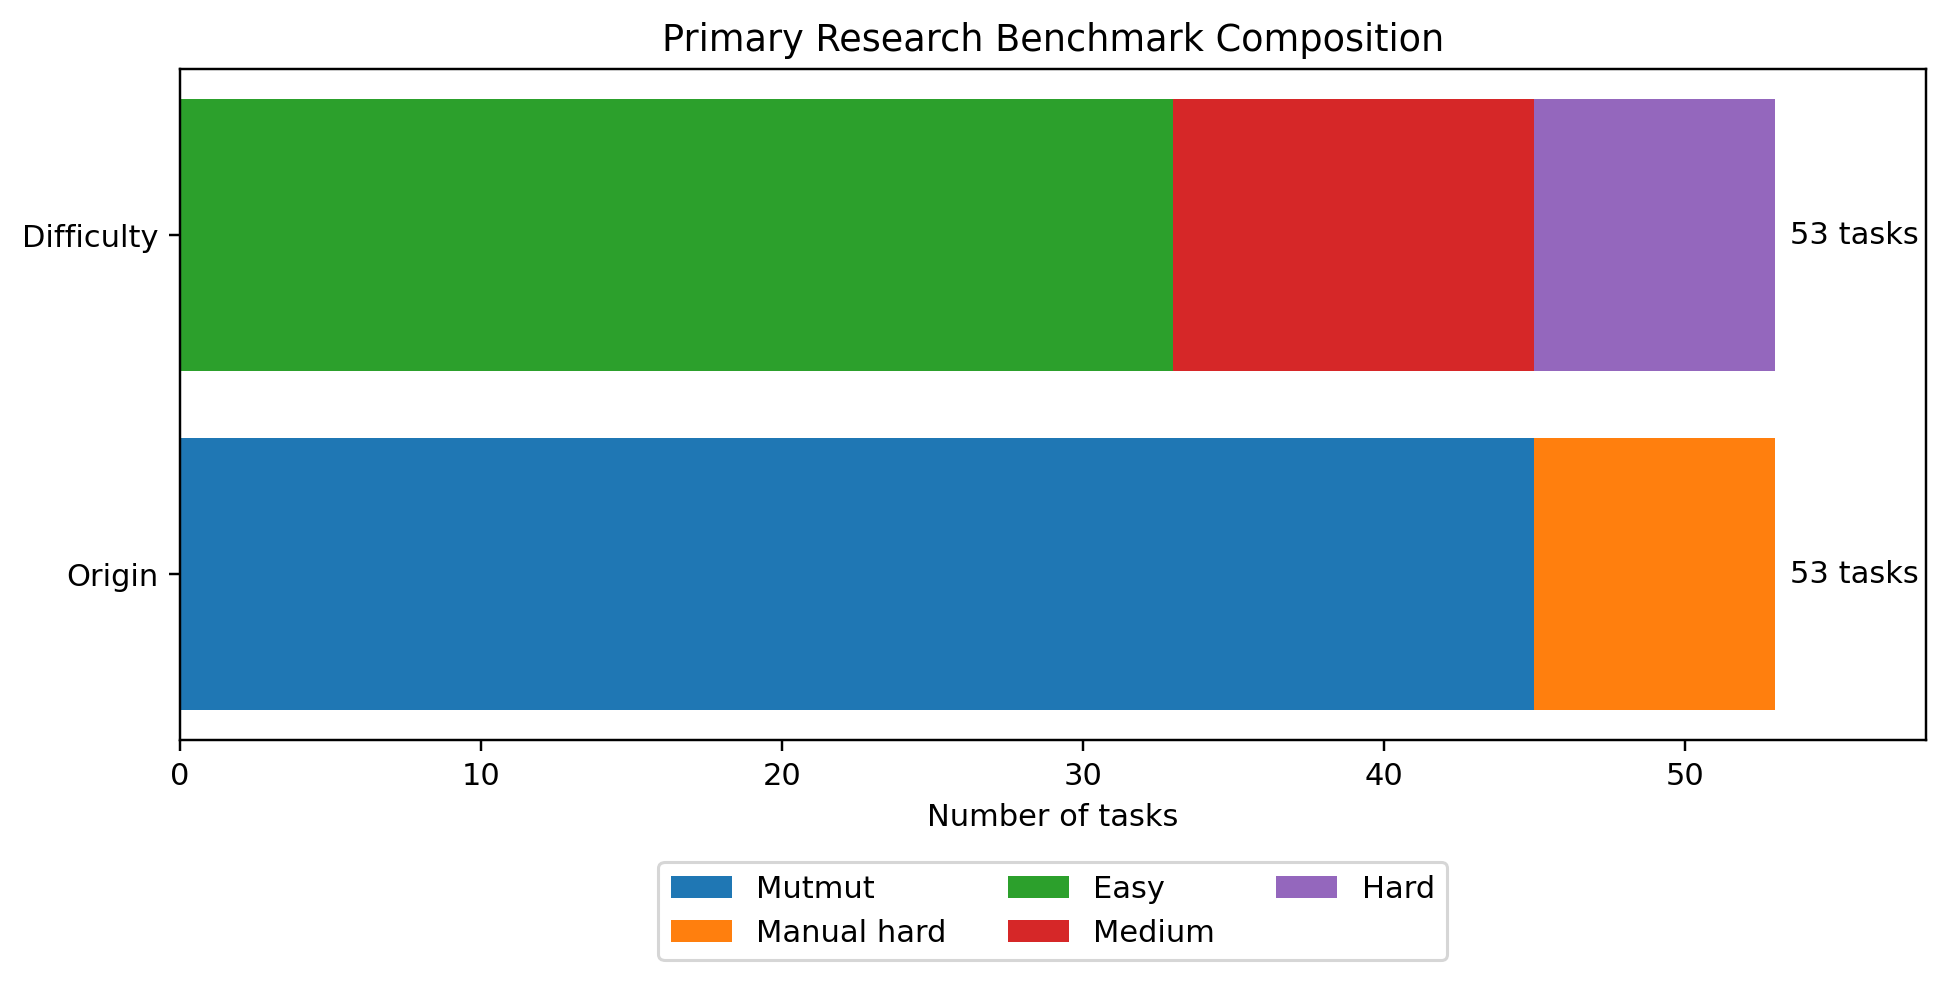
\includegraphics[width=0.82\textwidth]{assets/benchmark_composition.png}
\caption{Composition of the 53-task primary research benchmark.}
\label{fig:benchmark-composition}
\end{figure}

The proposal anticipated approximately 12--18 tasks; the final study uses 53
primary tasks and includes a separate set of hard cases. The hard set is not
mutation-generated and is therefore useful for exposing the model's capability
ceiling on multi-line, stateful defects.

\subsection{Conditions}

\begin{table}[H]
\centering
\caption{Canonical experimental conditions.}
\small
\begin{tabularx}{\textwidth}{p{0.20\textwidth}p{0.17\textwidth}p{0.15\textwidth}X}
\toprule
Condition & Tool selection & Retry / reflection & Operational definition \\
\midrule
One-shot & Runtime workflow & One patch; no retry & One model-generated repair
followed by syntax and full-suite verification. \\
Fixed workflow & Deterministic & Retry enabled; no reflection & Predetermined
staged sequence with model-generated patches and bounded retries. \\
Tool agent without reflection & Model selects among bounded tools & Retry enabled;
reflection forced null & Dynamic legal-action set with runtime-owned safety
transitions. \\
Full reflective agent & Model selects among bounded tools & Reflection required
after failed verification and rollback & Same bounded interface, plus a critique
and revised hypothesis before another repair attempt. \\
\bottomrule
\end{tabularx}
\end{table}

One-shot allows at most one patch and eight steps/tool calls. The other conditions
allow up to five patch attempts, 20 steps, and 30 tool calls, with a maximum
condition budget of 1,800 seconds.

\subsection{Model and reproducibility configuration}

All conditions use \code{qwen2.5-coder:3b} through Ollama with temperature 0,
seed 42, a requested maximum of 512 output tokens, a 300-second model timeout,
and a 60-second test timeout. One warmed model instance is shared across
conditions. The evaluation is tied to Git commit
\code{6524a37d802fc83faa9db0111facaf491da4e618} and completed with exit code
zero. The result matrix contains exactly 212 rows with no missing
task--condition pair.

\subsection{Metrics and statistical analysis}

The primary endpoint is hidden-verified repair success. Visible full-suite
success is reported separately to identify overfitting or test weakness.
Trajectory metrics include model calls, steps, tool calls, patch attempts,
decision-parse failures, invalid patches, no-progress rejections, rollback,
latency, and reflection events.

Matched binary outcomes are compared with Cochran's $Q$. The six planned
pairwise comparisons use exact McNemar tests with Holm correction
\cite{mcnemar,holm}. Wilson intervals summarize condition rates. Task-level
latencies use Friedman's test and paired Wilcoxon signed-rank tests with Holm
correction. Stratified origin and difficulty analyses are exploratory.

\clearpage
\section{Results}

\subsection{Primary repair outcomes}

\begin{table}[H]
\centering
\caption{Final repair outcomes. Hidden verification is the primary endpoint.}
\small
\begin{tabular}{lrrrr}
\toprule
Condition & Hidden verified & 95\% Wilson CI & Visible success & Mean time \\
\midrule
One-shot & 37/53 (69.8\%) & 56.5--80.5\% & 38/53 (71.7\%) & 86.5 s \\
Fixed workflow & 37/53 (69.8\%) & 56.5--80.5\% & 38/53 (71.7\%) & 105.7 s \\
Tool agent without reflection & 31/53 (58.5\%) & 45.1--70.7\% & 33/53 (62.3\%) & 350.1 s \\
Full reflective agent & 34/53 (64.2\%) & 50.7--75.7\% & 36/53 (67.9\%) & 249.6 s \\
\bottomrule
\end{tabular}
\end{table}

\begin{figure}[H]
\centering
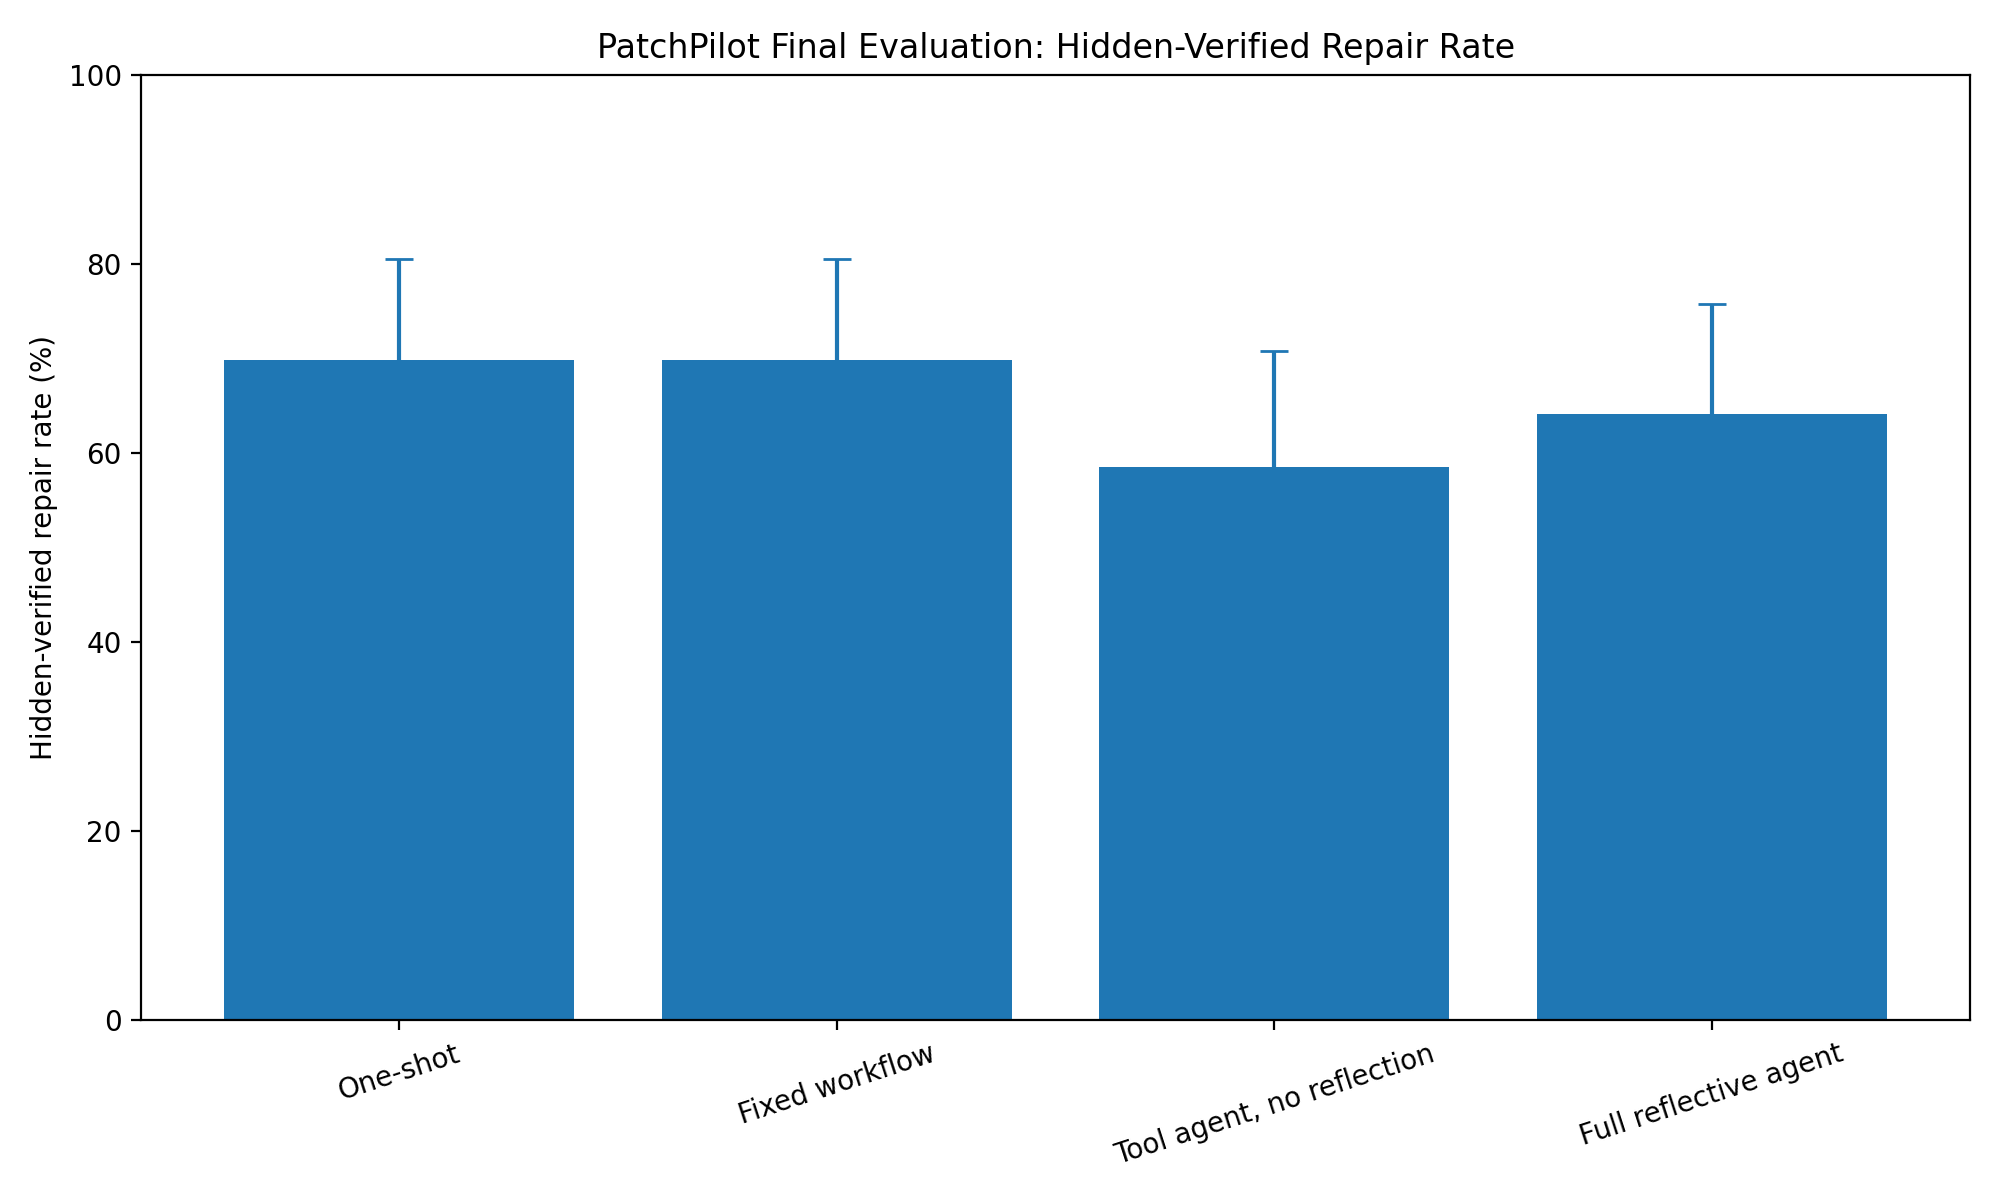
\includegraphics[width=0.88\textwidth]{assets/hidden_verified_rates_ci95.png}
\caption{Hidden-verified repair rates with 95\% Wilson intervals.}
\label{fig:main-results}
\end{figure}

Cochran's global test rejects equal success probabilities across all four
conditions: $Q(3)=11.000$, $p=0.0117$. This indicates heterogeneity within the matched four-condition set but does
not identify a specific superior pair.

\begin{table}[H]
\centering
\caption{Exact paired McNemar tests on hidden-verified success. ``A only'' means
a task solved by the first condition but not the second.}
\scriptsize
\resizebox{\textwidth}{!}{%
\begin{tabular}{lrrrrr}
\toprule
Comparison & A only & B only & Risk difference & Raw $p$ & Holm $p$ \\
\midrule
One-shot vs. Fixed workflow & 0 & 0 & +0.0 pp & 1.0000 & 1.0000 \\
One-shot vs. Tool agent without reflection & 6 & 0 & +11.3 pp & 0.0312 & 0.1875 \\
One-shot vs. Full reflective agent & 3 & 0 & +5.7 pp & 0.2500 & 1.0000 \\
Fixed workflow vs. Tool agent without reflection & 6 & 0 & +11.3 pp & 0.0312 & 0.1875 \\
Fixed workflow vs. Full reflective agent & 3 & 0 & +5.7 pp & 0.2500 & 1.0000 \\
Tool agent without reflection vs. Full reflective agent & 3 & 6 & -5.7 pp & 0.5078 & 1.0000 \\
\bottomrule
\end{tabular}}
\end{table}

No pairwise comparison remains significant after correction. The strongest
uncorrected contrast is one-shot versus the tool agent without reflection:
six tasks are solved only by one-shot and none only by the tool agent
(raw $p=0.0313$, Holm $p=0.1875$). One-shot and fixed workflow have identical
hidden-success vectors on all 53 tasks.

\subsection{Origin and difficulty}

\begin{table}[H]
\centering
\caption{Hidden-verified success by benchmark origin.}
\begin{tabular}{lrr}
\toprule
Condition & Mutmut tasks ($n=45$) & Manual hard tasks ($n=8$) \\
\midrule
One-shot & 37/45 (82.2\%) & 0/8 (0.0\%) \\
Fixed workflow & 37/45 (82.2\%) & 0/8 (0.0\%) \\
Tool agent without reflection & 31/45 (68.9\%) & 0/8 (0.0\%) \\
Full reflective agent & 34/45 (75.6\%) & 0/8 (0.0\%) \\
\bottomrule
\end{tabular}
\end{table}

\begin{figure}[H]
\centering
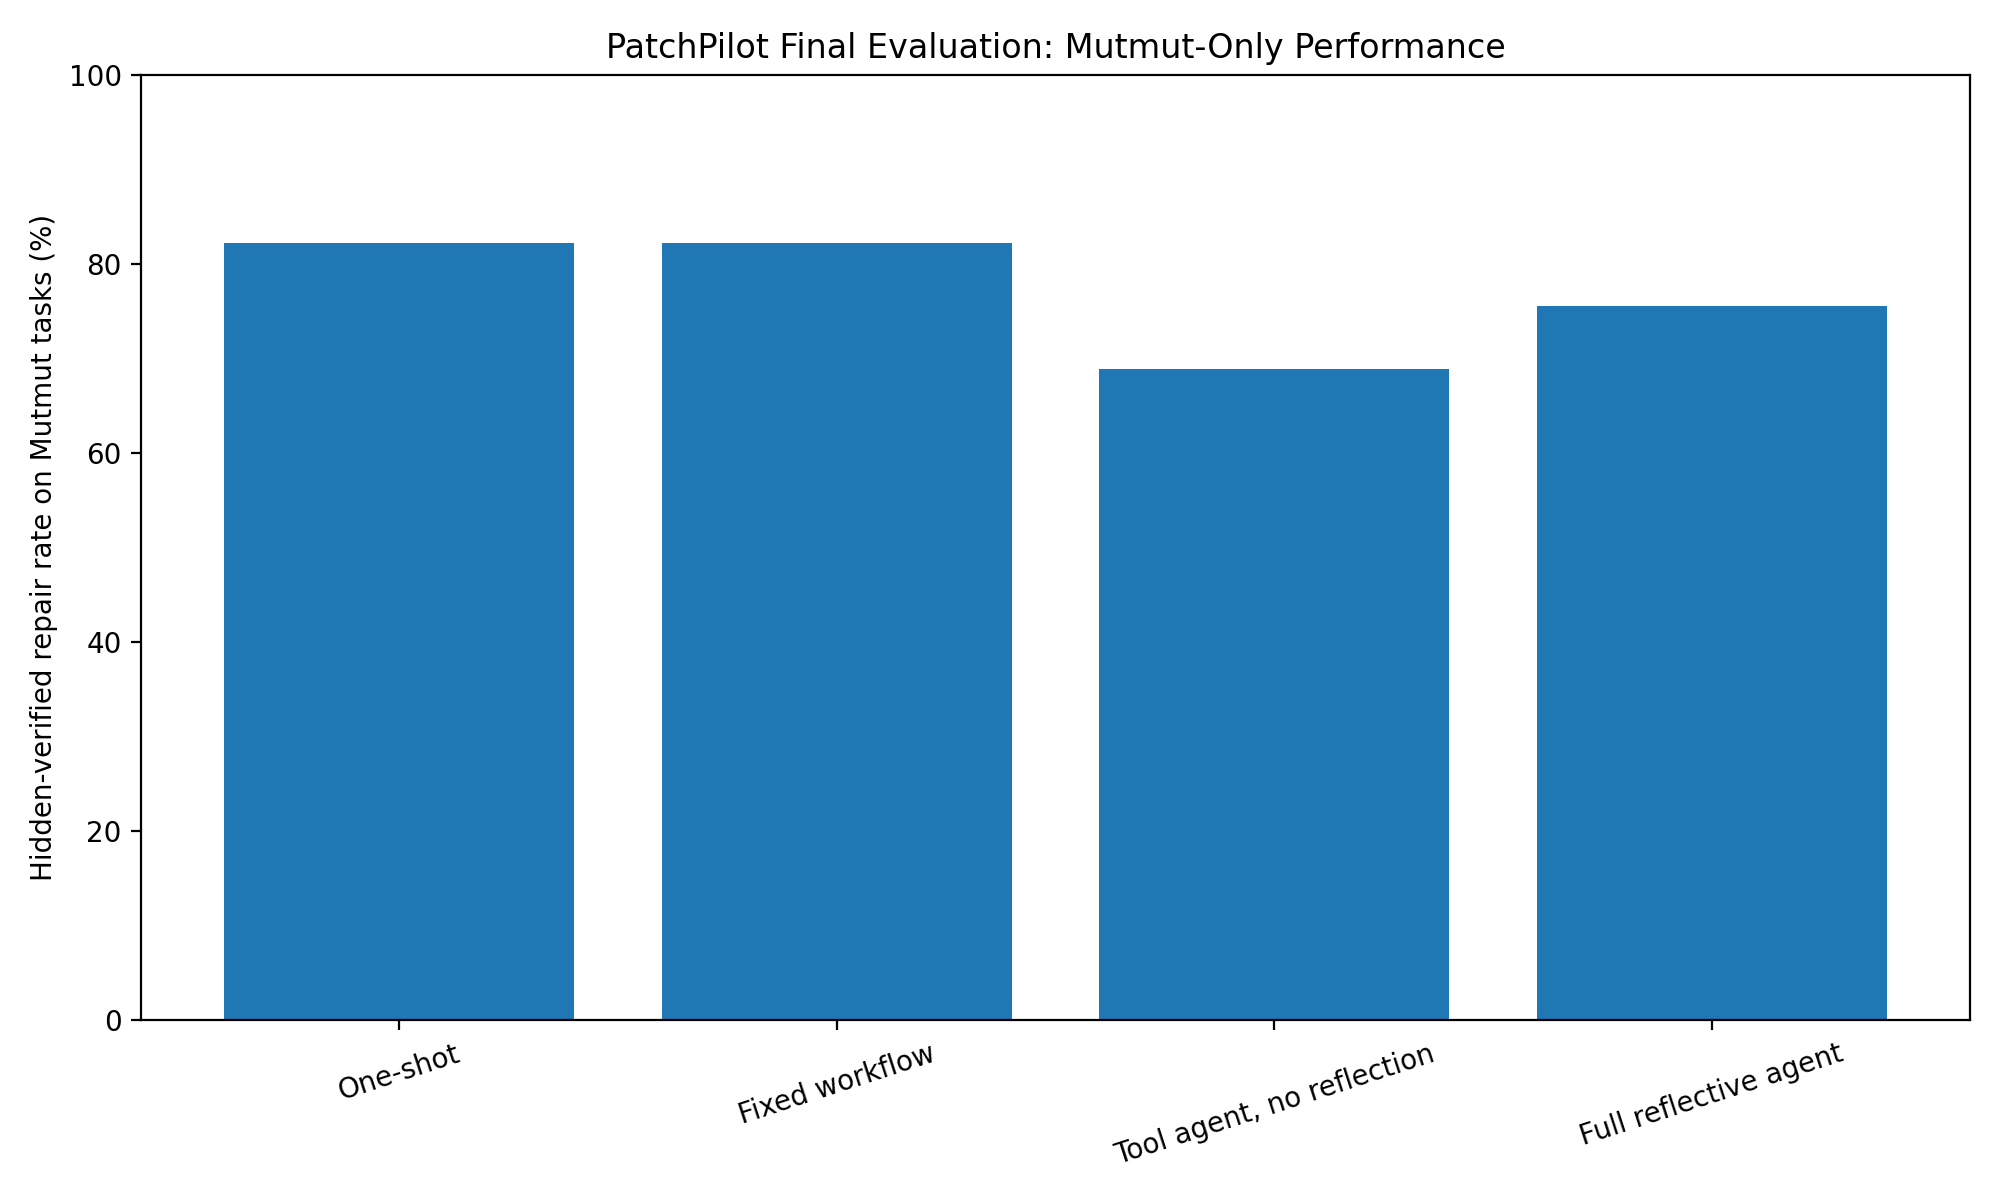
\includegraphics[width=0.88\textwidth]{assets/mutmut_hidden_verified_rates.png}
\caption{Hidden-verified performance on the 45 mutation-generated tasks.}
\end{figure}

All four conditions score 0/8 on the manual hard challenges. Therefore, every
difference in the aggregate score comes from the mutation-generated tasks.
Within this benchmark, the result marks a capability limit for the 3B model
and the current repair interface.

\begin{table}[H]
\centering
\caption{Hidden-verified success by assigned task difficulty.}
\begin{tabular}{lrrr}
\toprule
Condition & Easy ($n=33$) & Medium ($n=12$) & Hard ($n=8$) \\
\midrule
One-shot & 26/33 (78.8\%) & 11/12 (91.7\%) & 0/8 (0.0\%) \\
Fixed workflow & 26/33 (78.8\%) & 11/12 (91.7\%) & 0/8 (0.0\%) \\
Tool agent without reflection & 21/33 (63.6\%) & 10/12 (83.3\%) & 0/8 (0.0\%) \\
Full reflective agent & 25/33 (75.8\%) & 9/12 (75.0\%) & 0/8 (0.0\%) \\
\bottomrule
\end{tabular}
\end{table}

Medium tasks outperform easy tasks for the two baselines because difficulty is a
benchmark metadata label and the selected task families differ; the pattern
should not be generalized beyond this suite.

\subsection{Efficiency and trajectory cost}

\begin{table}[H]
\centering
\caption{Trajectory and efficiency metrics per run.}
\scriptsize
\resizebox{\textwidth}{!}{%
\begin{tabular}{lrrrrrr}
\toprule
Condition & Model calls & Steps & Parse-failure runs & Policy failures &
Mean seconds & Seconds per hidden success \\
\midrule
One-shot & 1.15 & 5.58 & 9 & 6 & 86.5 & 123.9 \\
Fixed workflow & 1.47 & 5.81 & 15 & 15 & 105.7 & 151.5 \\
Tool agent without reflection & 3.96 & 5.40 & 21 & 20 & 350.1 & 598.6 \\
Full reflective agent & 3.53 & 5.58 & 16 & 17 & 249.6 & 389.1 \\
\bottomrule
\end{tabular}}
\end{table}

\begin{figure}[H]
\centering
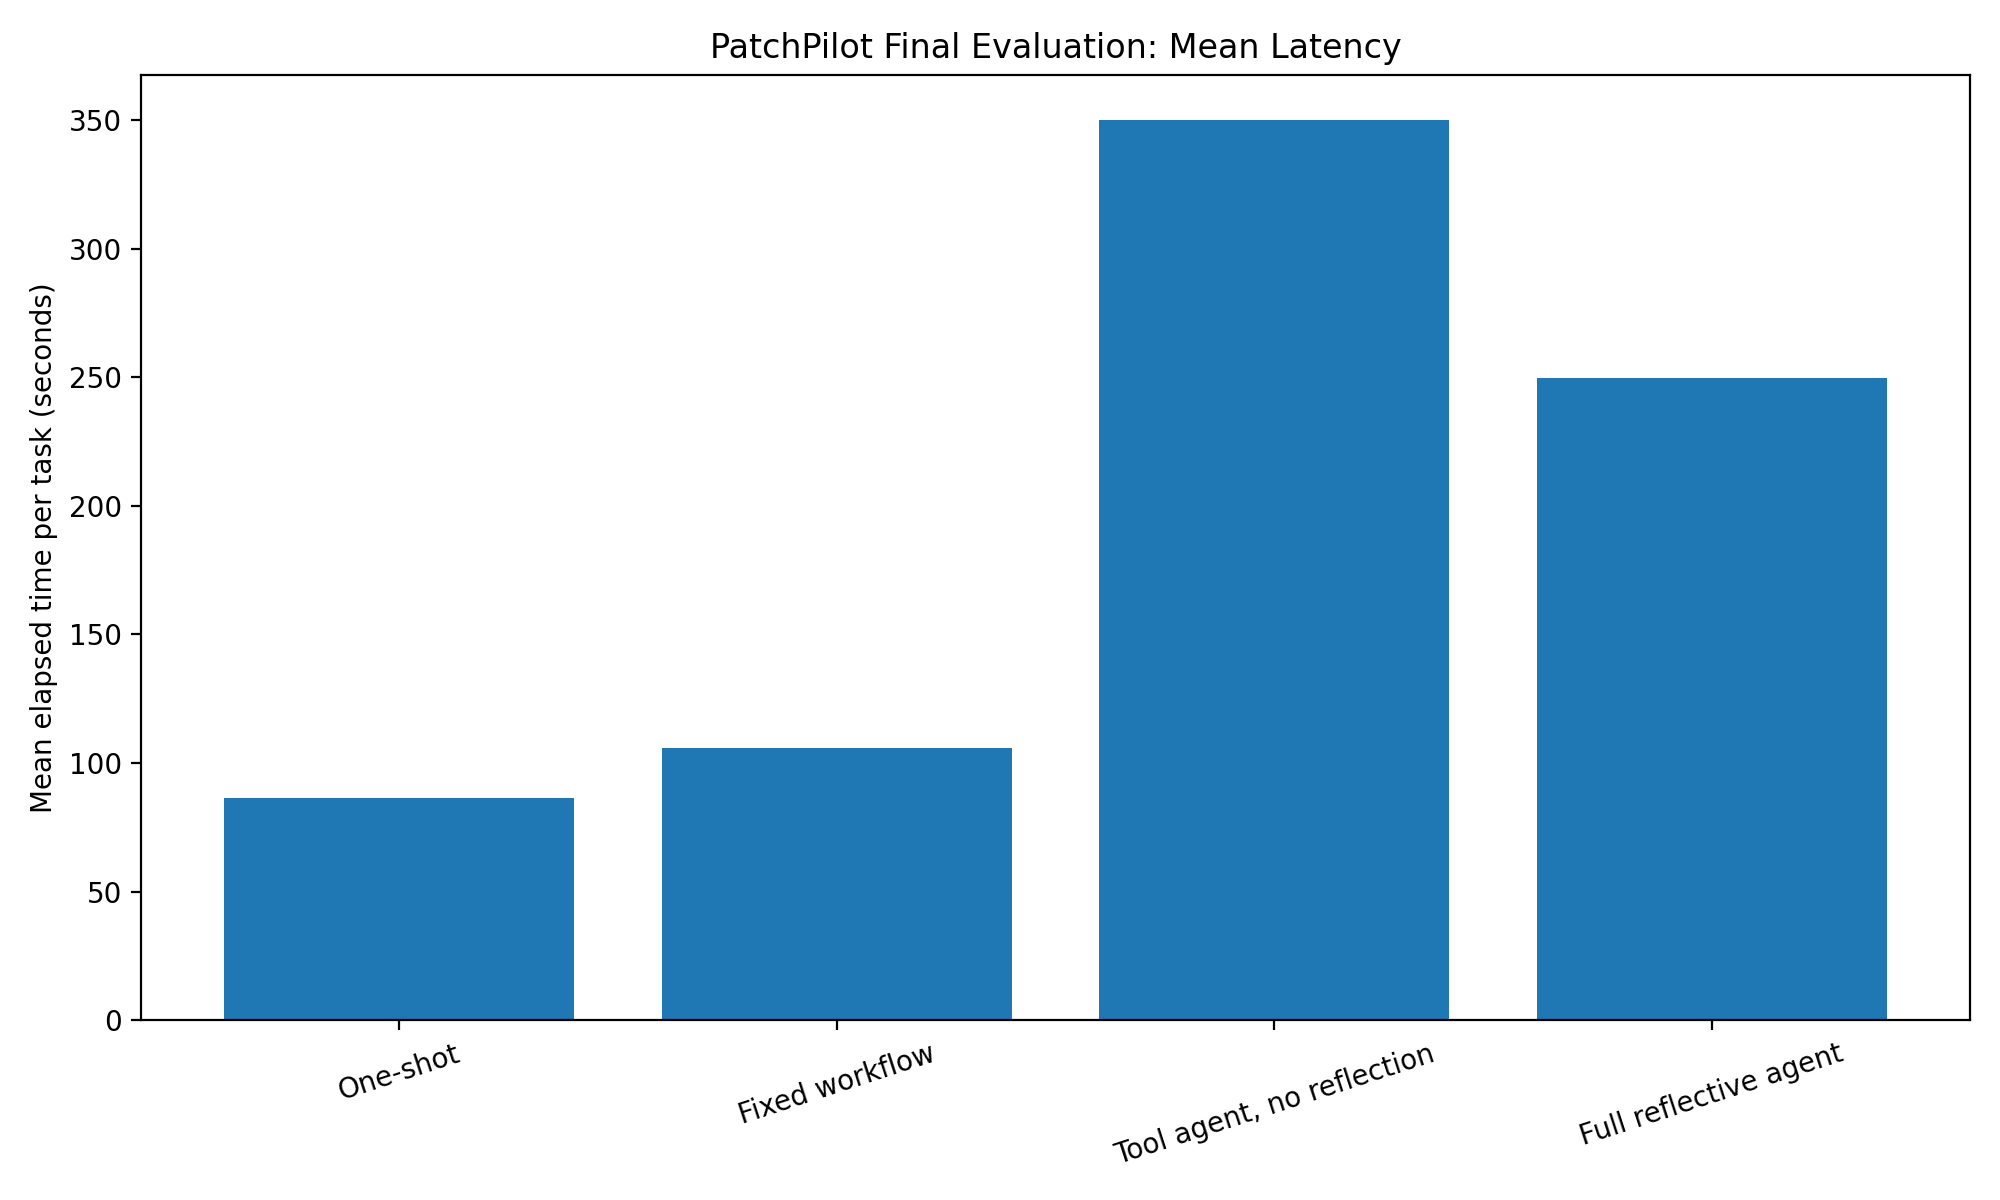
\includegraphics[width=0.88\textwidth]{assets/mean_latency_by_condition.png}
\caption{Mean elapsed time per task.}
\label{fig:latency}
\end{figure}

Latency differs strongly across matched tasks
($\chi^2_F(3)=143.785$, $p=5.77\times10^{-31}$). All six paired Wilcoxon
comparisons remain significant after Holm correction. Mean latency orders the
conditions as one-shot, fixed workflow, reflective agent, then non-reflective
tool agent. Compared with one-shot, the reflective configuration is 2.89 times
slower and the non-reflective tool agent is 4.05 times slower.

The fixed workflow produces exactly the same hidden outcomes as one-shot while
taking 22\% longer on average. In this run, retry capability did not recover any
task that one-shot missed.

\subsection{Decision parsing and failure localization}

\begin{table}[H]
\centering
\caption{Hidden-success rates conditional on decision-parse failures. Fisher
tests are descriptive because difficulty can affect both parsing and success.}
\small
\resizebox{0.96\textwidth}{!}{%
\begin{tabular}{lrrrr}
\toprule
Condition & Parse-failure runs & Success with failure & Success without failure &
Fisher $p$ \\
\midrule
One-shot & 9 & 11.1\% & 81.8\% & 1.10e-04 \\
Fixed workflow & 15 & 6.7\% & 94.7\% & 7.13e-10 \\
Tool agent without reflection & 21 & 4.8\% & 93.8\% & 2.26e-11 \\
Full reflective agent & 16 & 0.0\% & 91.9\% & 6.53e-11 \\
\bottomrule
\end{tabular}}
\end{table}

\begin{figure}[H]
\centering
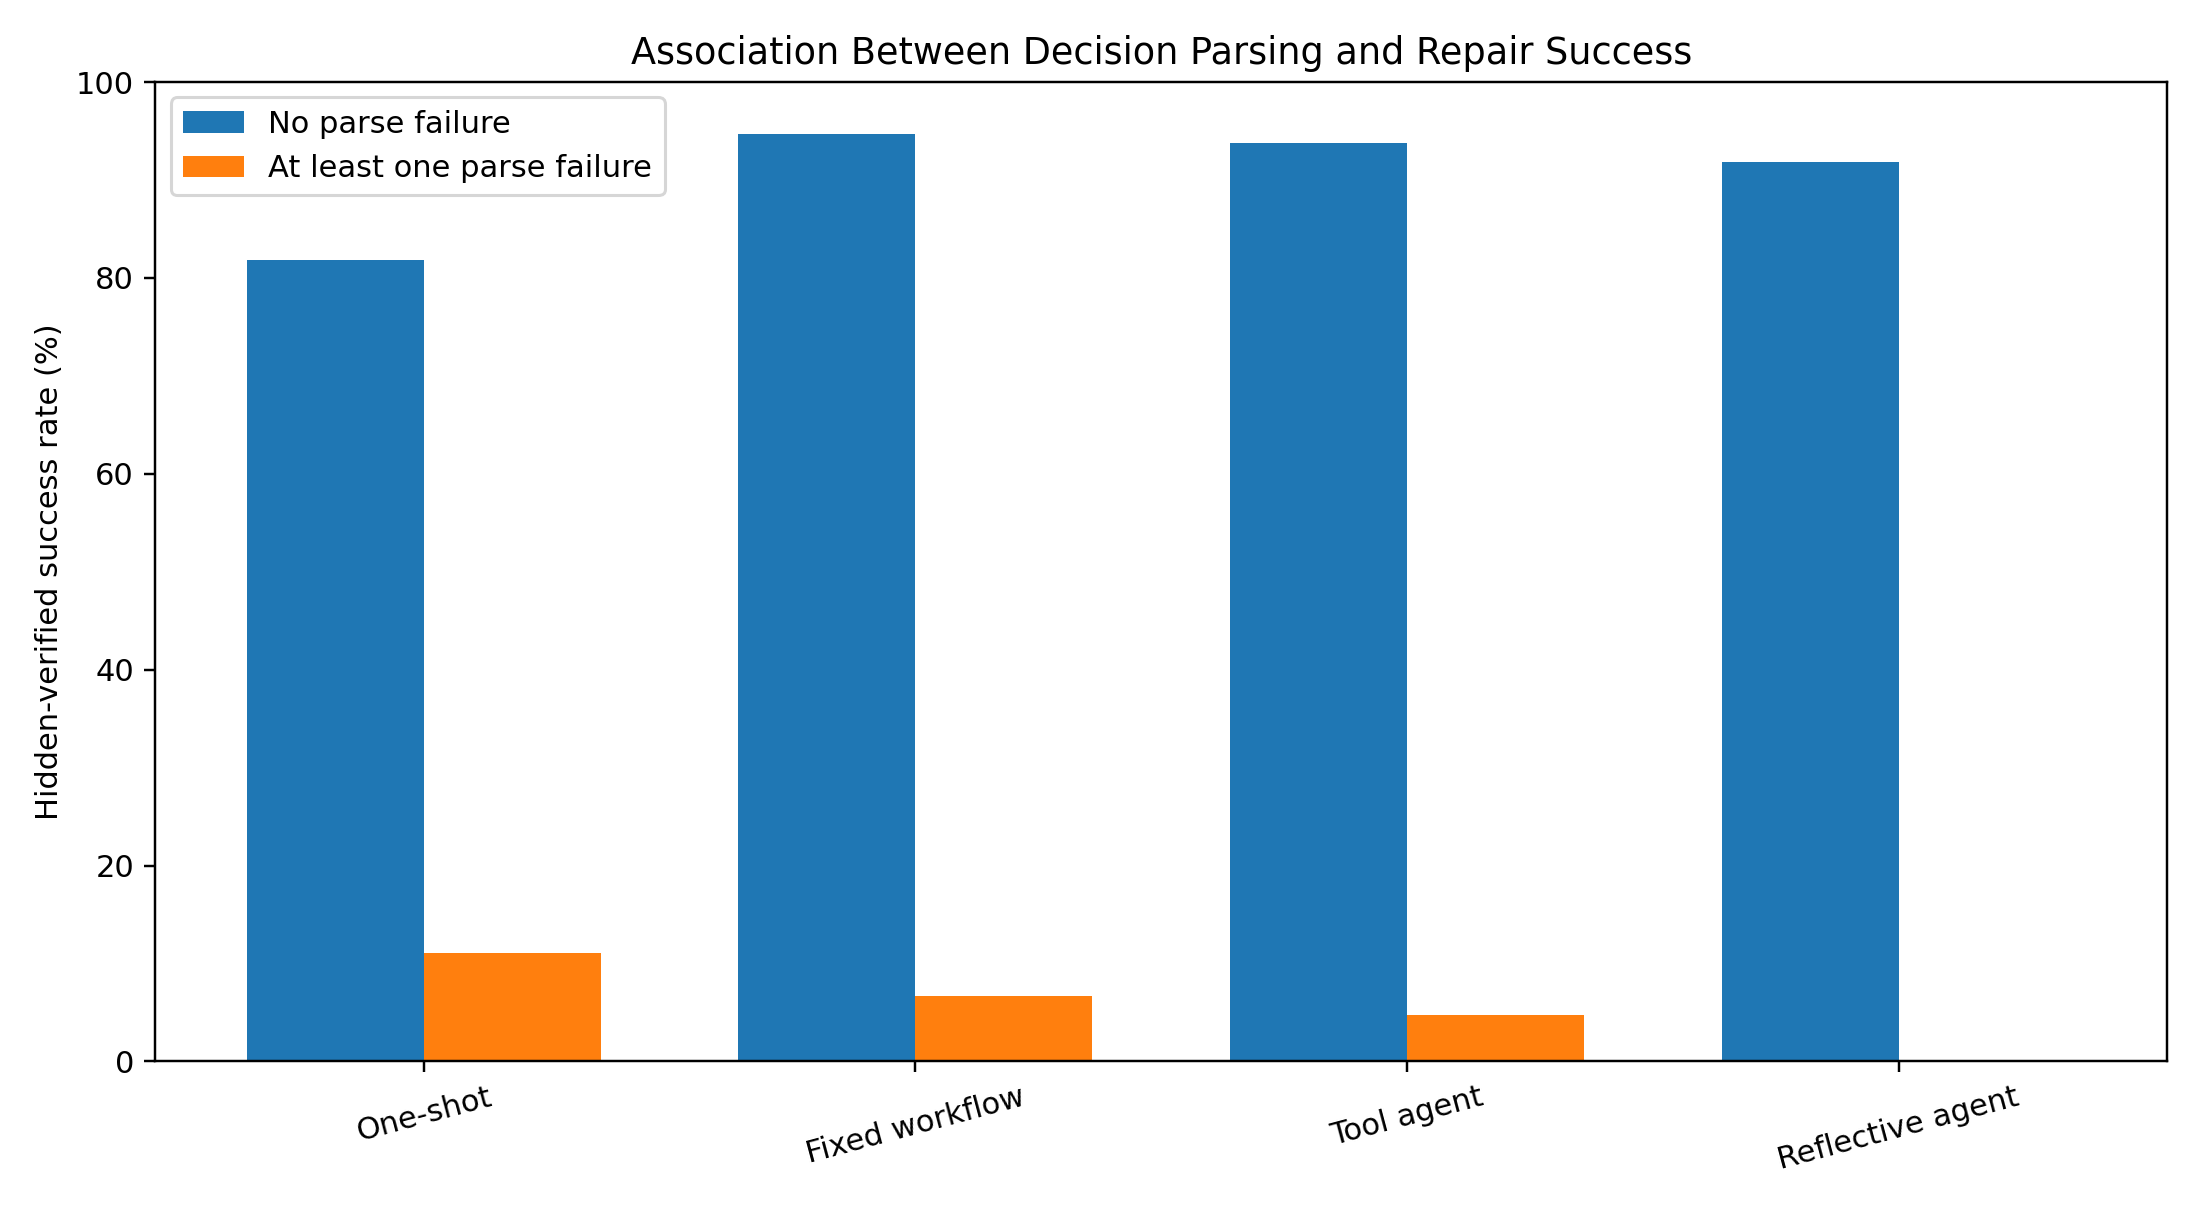
\includegraphics[width=0.88\textwidth]{assets/parse_failure_success_rates.png}
\caption{Repair success is associated with structured-output reliability. The
association is descriptive and is not interpreted as causal.}
\end{figure}

The original navigation-loop defect is no longer present: there are zero budget
exhaustions, zero invalid-patch runs, and zero no-progress-loop runs. The
remaining escalations are dominated by decision-parse errors: six one-shot,
15 fixed-workflow, 20 non-reflective-agent, and 17 reflective-agent runs.
In the recorded trajectories, decision parsing is the most frequent remaining
failure category; unsafe patch execution and budget loops were not observed.

\subsection{Hidden verification and visible disagreement}

Six runs pass visible verification but fail hidden verification. The
\code{clamp} task disagrees in all four conditions; one text parsing task
disagrees only for the non-reflective agent and another only for the reflective
agent. Hidden success is therefore the appropriate primary metric. No run is
counted as an unverified success.

\subsection{Reflection ablation result}

The configured reflective condition achieves 34 hidden successes versus 31 for
the non-reflective tool agent. Their paired outcomes contain six tasks solved
only by the reflective condition and three only by the non-reflective condition
(exact McNemar $p=0.5078$, Holm $p=1.0$).

However, the reflective traces record \textbf{zero completed reflection events}
and \textbf{zero hypothesis revisions}. Failed runs generally terminate during
decision parsing before a completed failed-patch--rollback--reflection cycle.
Accordingly, the observed difference cannot be attributed causally to
reflection. The experiment evaluates two configured policies, but it does not
provide process evidence that verbal reflection was exercised.

\clearpage
\section{Demonstration Interface}

The Streamlit application is a live repair demonstration rather than a chat
interface. Users select a benchmark family and task, inspect source and regression
tests, choose a local Ollama model, run the repair pipeline, and review
verification, the action trajectory, and the generated diff. The validated 3B
model is the default. A compact evidence expander reports the final 212-run
evaluation without turning the demonstration into a static dashboard.

\begin{figure}[H]
\centering
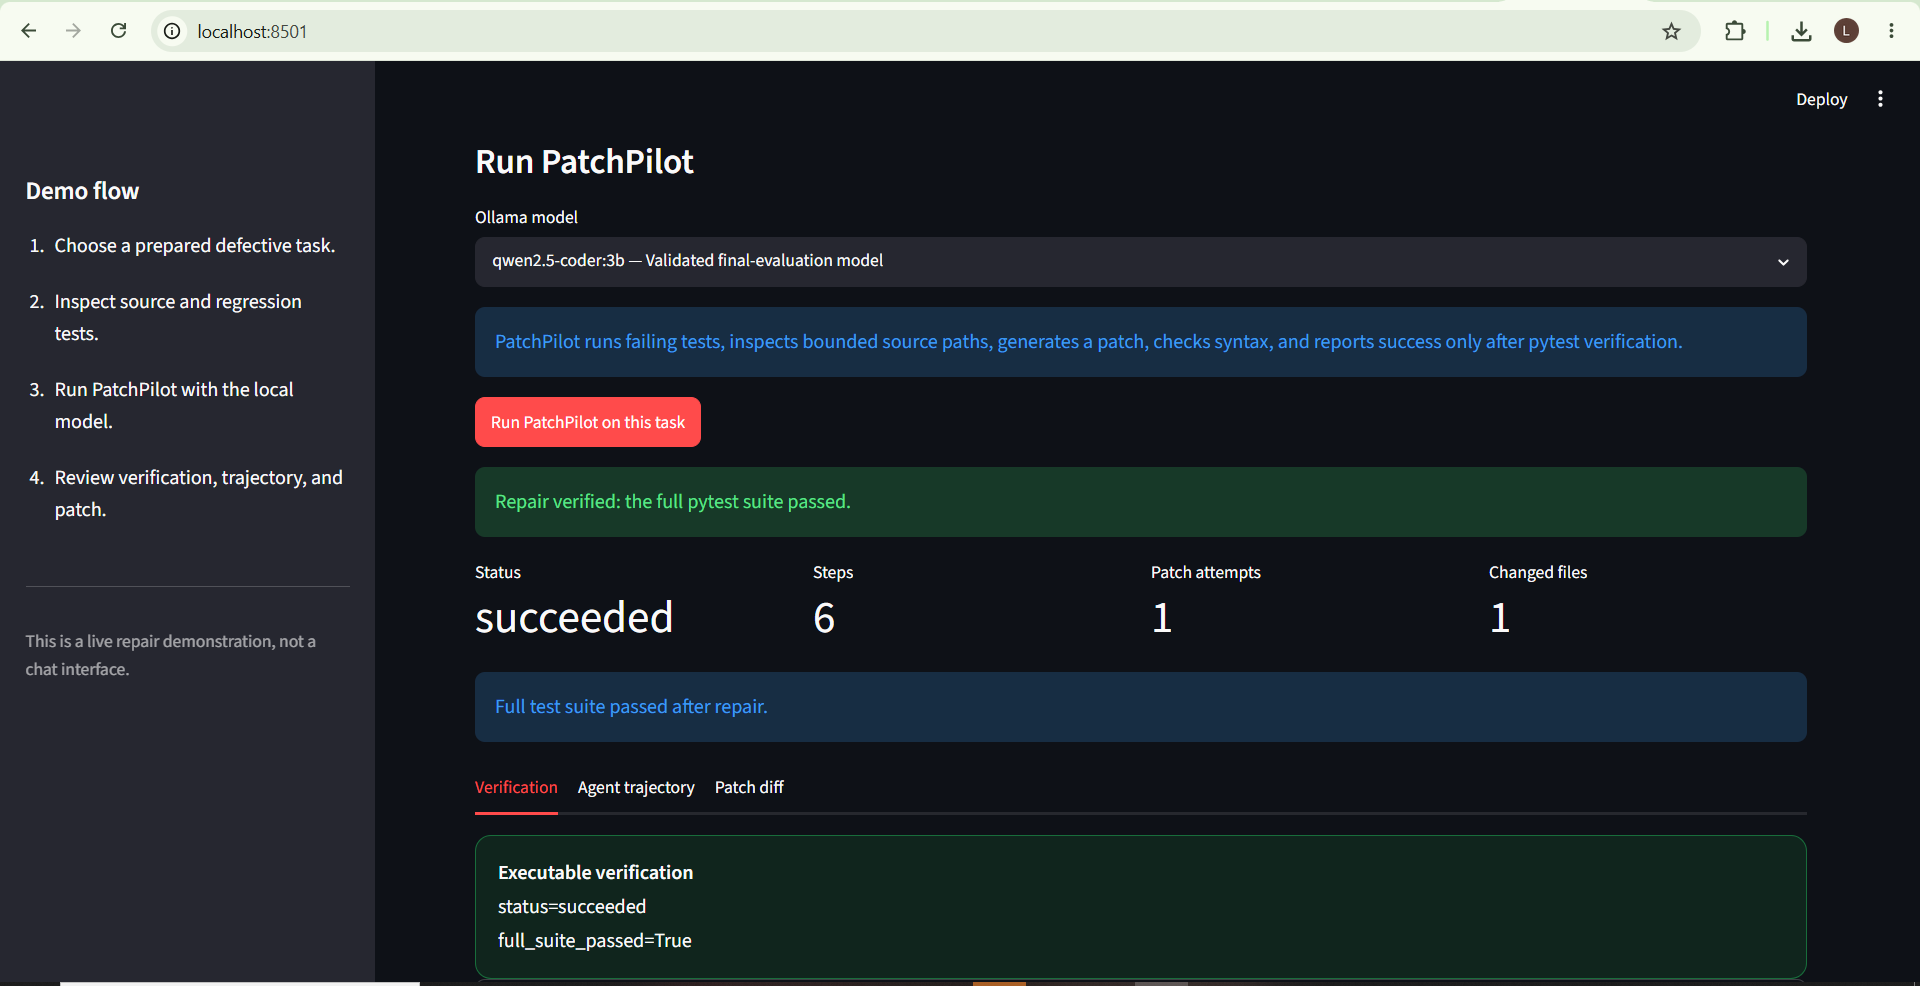
\includegraphics[width=0.98\textwidth]{assets/patchpilot_verified_live_repair.png}
\caption{Completed live repair demonstration. The page shows the validated
model, successful status, six steps, one patch attempt, one changed file, and
full pytest verification.}
\label{fig:ui}
\end{figure}

\clearpage
\section{Discussion}

\subsection{Answer to the research questions}

\textbf{RQ1.} The four conditions have different aggregate hidden outcomes,
but no planned pair is significant after multiple-comparison correction.
One-shot and fixed workflow tie for the highest observed rate.

\textbf{RQ2.} The reflective configuration exceeds the non-reflective tool
agent descriptively, but not significantly. Because no reflection events or
hypothesis revisions occur, the experiment does not establish the effect of
reflection itself.

\textbf{RQ3.} Additional agency is costly. Tool agents require roughly three to
four model calls per task and are 2.9--4.0 times slower than one-shot. Parsing
reliability, rather than patch safety or budget loops, is the dominant remaining
trajectory problem.

\textbf{RQ4.} In the evaluated suite, the runtime recorded zero invalid-patch runs, zero
no-progress runs, zero budget exhaustions, and no unverified successes. These
are observations for this experiment and do not imply that the model cannot
propose incorrect code.

\subsection{Why simpler conditions performed best}

The result illustrates that greater autonomy does not automatically produce
better repair. The 3B model is strong enough to solve many local mutations from a
compact evidence prompt, but additional structured decisions introduce more
opportunities for parse failure and latency. The fixed workflow adds retry
overhead without recovering any additional task. The tool agents retain model
choice, but the small model spends more calls producing structured actions and
remains unable to solve the hard stateful tasks.

The result is consistent with the course observation that additional test-time
reasoning can reduce performance when
the critic, planner, or interface is unreliable \cite{courseplanning}. It also
supports the ACI perspective: reliable interfaces and concise evidence can be as
important as nominal agent autonomy.

\subsection{Contributions}

The implemented project includes:

\begin{itemize}
  \item a typed, safety-constrained agent-computer interface for Python repair;
  \item model-selected bounded tools with executor-derived argument schemas;
  \item isolated workspaces, protected tests, syntax gates, revision-aware
  verification, and transactional rollback;
  \item append-only trajectory traces and post-run hidden verification;
  \item a 53-task benchmark spanning mutation defects and eight hard manual
  challenges;
  \item a 212-run four-condition evaluation with paired statistics;
  \item a reproducible analysis script, committed result tables and charts, and
  a live Streamlit repair demonstration.
\end{itemize}

\Needspace{10\baselineskip}
\section{Project Requirements Alignment}

\begin{table}[H]
\centering
\caption{Implemented deliverables compared with the original proposal.}
\small
\begin{tabularx}{\textwidth}{>{\raggedright\arraybackslash}p{0.27\textwidth}>{\raggedright\arraybackslash}p{0.14\textwidth}>{\raggedright\arraybackslash}X}
\toprule
Proposal item & Status & Evidence in this report \\
\midrule
Single-agent Plan--Act--Observe--Reflect--Verify workflow & Partially
demonstrated & Plan/action/observation/verification are implemented and traced;
the reflective policy exists, but final trajectories record no completed
reflection cycle. \\
Restricted repository tools, syntax checks, diff inspection, rollback &
Implemented & Nine exact-schema tools, protected tests, syntax gate,
transactional restoration, and current-revision verification. \\
Isolated execution, allow-lists, time and tool budgets & Implemented & Fresh
workspaces, restricted pytest execution, per-condition budgets, model and test
timeouts. \\
Approximately 12--18 repair tasks & Expanded & 53 primary tasks: 45 Mutmut and
eight hard manual challenges; 12 sanity tasks excluded. \\
Four baseline and ablation conditions & Implemented & One-shot, fixed workflow,
tool agent without reflection, and full reflective agent. \\
Repair, safety, attempts, tools, time, rollback, and budget metrics &
Implemented & Run-level CSV, hidden verification, trajectory counts, paired
statistics, and reproducible analysis. \\
Simple demonstration interface & Implemented & Live Streamlit task inspection,
repair execution, trace, diff, and pytest verification. \\
Auditable repository and final technical report & Implemented & Signed commits,
274 passing tests at reporting time, Ruff, mypy, committed result assets, and
this report package. \\
\bottomrule
\end{tabularx}
\end{table}

\Needspace{10\baselineskip}
\section{Limitations and Threats to Validity}

\begin{itemize}
  \item \textbf{Single model and seed.} The final matrix uses one local
  3B model configuration with temperature zero and one seed. The results
  characterize the complete system configuration, not all code models.
  \item \textbf{Benchmark composition.} Forty-five of 53 tasks are synthetic
  mutation defects in small repositories. This provides reproducibility but
  limits external validity.
  \item \textbf{Hard-task ceiling.} Every condition fails all eight manual
  challenges. The interface and model do not yet support robust multi-file,
  long-horizon, or protocol-level reasoning.
  \item \textbf{Reflection not activated.} The reflective condition's intended
  mechanism is not observed in the final trajectories, so its causal effect
  cannot be estimated.
  \item \textbf{Structured-output sensitivity.} Parse errors remain associated with terminal failure, especially in the
  agentic conditions.
  \item \textbf{No repeated stochastic trials.} Paired task comparisons improve
  internal control, but repeated runs across seeds would better estimate
  variability.
  \item \textbf{Hidden tests are still benchmark-specific.} Hidden verification
  reduces visible-test overfitting but does not guarantee semantic correctness
  outside the defined test suites.
  \item \textbf{Naming overlap.} The independently developed project shares a name with Li et al.'s system.
  This report distinguishes the two through explicit citation and description.
\end{itemize}

\Needspace{10\baselineskip}
\section{Future Work}

A useful next step is a benchmark that exercises failed-patch recovery and
records completed reflection and hypothesis-revision cycles. Stronger structured-output
models or constrained decoding should be compared without changing the
agent-computer interface. Repeated seeds and multiple local model sizes would
separate model variance from scaffold effects.

Longer-term extensions include ranked fault localization, richer evidence
summaries, multi-file patches, dependency-aware environments, parallel
investigation, and evaluation on fresh real-issue benchmarks. The trajectory
analysis should remain part of continuous integration so that changes are judged
on correctness, cost, safety, and tool reliability rather than repair rate
alone.

\Needspace{10\baselineskip}
\section{Reproducibility and Software Quality}

The final evaluation began on July 14, 2026 and completed on July 15 with 212/212
runs and exit code zero. The experiment configuration, run-level CSV, summaries,
hashes, figures, and statistical outputs are stored under
\path{results/final-research-evaluation-6524a37/}. The script
\path{scripts/analyze_final_evaluation.py} reproduces Cochran's $Q$, exact
McNemar comparisons, Wilson intervals, and summary artifacts.

At reporting time the repository quality gates report 274 tests passed, Ruff
passed, mypy reported no issues across 32 source files, and
\code{git diff --check} passed. Commits are signed and the evaluated repair
runtime is preserved at \code{6524a37}.

\begin{lstlisting}[basicstyle=\ttfamily\small,frame=single,
breaklines=true]
python -m pip install -e ".[dev,analysis]"
python -m ruff check .
python -m pytest -q
python -m mypy src

python scripts/analyze_final_evaluation.py \
  artifacts/evaluation/final-research-evaluation-6524a37-20260714-090253/runs.csv \
  --output-dir results/final-research-evaluation-6524a37/reproduced

streamlit run demo/streamlit_app.py --server.port 8501
\end{lstlisting}

\Needspace{10\baselineskip}
\section{Conclusion}

PatchPilot implements an end-to-end bounded repair prototype rather than an
unverified code-generation workflow. It interacts with real repositories through
restricted tools, protects tests, validates exact arguments, applies
transactional patches, tracks revisions, verifies with visible and hidden test
suites, records auditable trajectories, and exposes the workflow through a live
interface.

The empirical conclusion is intentionally modest. Under
\code{qwen2.5-coder:3b}, the simple one-shot and fixed-workflow conditions
achieve the highest observed hidden-verified repair rate. The configured
reflective agent improves descriptively over the non-reflective tool agent, but
no corrected pairwise difference is significant and no completed reflection
event is observed. Additional agency therefore increases latency without a
demonstrated outcome gain in this configuration.

The result is informative for subsequent system design. The evaluation
highlights hard stateful defects and structured-output reliability as current
bottlenecks, while documenting runtime constraints, reproducibility, and
trajectory observability around a small local model.

\clearpage
\clearpage
\section*{References}
\addcontentsline{toc}{section}{References}
\begin{thebibliography}{99}

\bibitem{react}
S. Yao, J. Zhao, D. Yu, N. Du, I. Shafran, K. Narasimhan, and Y. Cao.
\newblock ReAct: Synergizing Reasoning and Acting in Language Models.
\newblock \emph{International Conference on Learning Representations}, 2023.
\newblock \url{https://arxiv.org/abs/2210.03629}.

\bibitem{reflexion}
N. Shinn, F. Cassano, E. Berman, A. Gopinath, K. Narasimhan, and S. Yao.
\newblock Reflexion: Language Agents with Verbal Reinforcement Learning.
\newblock \emph{Advances in Neural Information Processing Systems}, 2023.
\newblock \url{https://arxiv.org/abs/2303.11366}.

\bibitem{sweagent}
J. Yang, C. E. Jimenez, A. Wettig, K. Lieret, S. Yao, K. Narasimhan,
and O. Press.
\newblock SWE-agent: Agent-Computer Interfaces Enable Automated Software
Engineering.
\newblock \emph{Advances in Neural Information Processing Systems}, 2024.
\newblock \url{https://arxiv.org/abs/2405.15793}.

\bibitem{swebench}
C. E. Jimenez, J. Yang, A. Wettig, S. Yao, K. Pei, O. Press,
and K. Narasimhan.
\newblock SWE-bench: Can Language Models Resolve Real-World GitHub Issues?
\newblock \emph{International Conference on Learning Representations}, 2024.
\newblock \url{https://arxiv.org/abs/2310.06770}.

\bibitem{externalpatchpilot}
H. Li, Y. Tang, S. Wang, and W. Guo.
\newblock PatchPilot: A Stable and Cost-Efficient Agentic Patching Framework.
\newblock arXiv:2502.02747, 2025.
\newblock \url{https://arxiv.org/abs/2502.02747}.

\bibitem{qwen}
B. Hui et al.
\newblock Qwen2.5-Coder Technical Report.
\newblock arXiv:2409.12186, 2024.
\newblock \url{https://arxiv.org/abs/2409.12186}.

\bibitem{quixbugs}
H. Ye, M. Martinez, T. Durieux, and M. Monperrus.
\newblock A Comprehensive Study of Automatic Program Repair on the QuixBugs
Benchmark.
\newblock \emph{Journal of Systems and Software}, 171:110825, 2021.
\newblock \url{https://arxiv.org/abs/1805.03454}.

\bibitem{mcnemar}
Q. McNemar.
\newblock Note on the Sampling Error of the Difference Between Correlated
Proportions or Percentages.
\newblock \emph{Psychometrika}, 12(2):153--157, 1947.

\bibitem{holm}
S. Holm.
\newblock A Simple Sequentially Rejective Multiple Test Procedure.
\newblock \emph{Scandinavian Journal of Statistics}, 6(2):65--70, 1979.

\bibitem{courseeval}
A. Sillitti.
\newblock Evaluation and Observability.
\newblock Agentic AI course lecture, Innopolis University, 2026.

\bibitem{courseplanning}
A. Sillitti.
\newblock Advanced Reasoning and Planning.
\newblock Agentic AI course lecture, Innopolis University, 2026.

\end{thebibliography}

\end{document}
